% mainfile: ../../../../master.tex
\subsection{DNA and RNA quantification with Qubit\texttrademark~ BR assays}
% The part of the label after the colon must match the file name. Otherwise,
% conditional compilation based on task labels does NOT work.
\label{task:20180213_cj3}
\tags{lab,dna,rna,qnt}
\authors{cj}
%\files{}
%\persons{}
\sidenote{Qubit dsDNA BR assay opened by Elísabet on 20170815; \texttt{LOT: 1835789}}
\sidenote{Qubit RNA BR assay opened by me on 20180209; \texttt{LOT: 1924395}}

\begin{figure}[H] % position of the figure 
    \centering
    \caption{Illustration for the Qubit\texttrademark~ assays}
    \label{fig:20180213_Qubit_assays}
    \begin{subfigure}[b]{0.49\textwidth}
        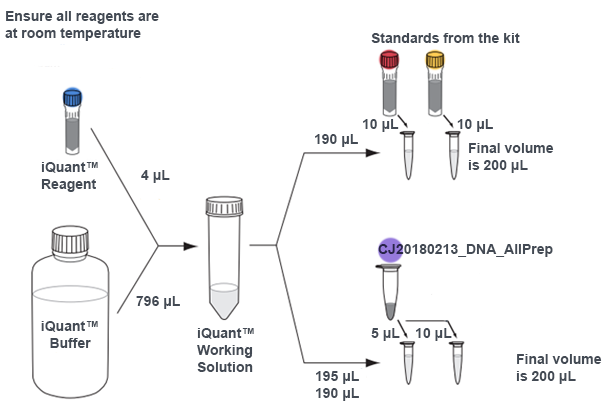
\includegraphics[width=\textwidth]{graphics/schemas/20180213_Qubit_assay_DNA.png}
        \caption{Qubit\texttrademark~ dsDNA BR assay}
        \label{sfig:20180213_Qubit_assay_DNA}
    \end{subfigure}
    ~ 
    \begin{subfigure}[b]{0.49\textwidth}
        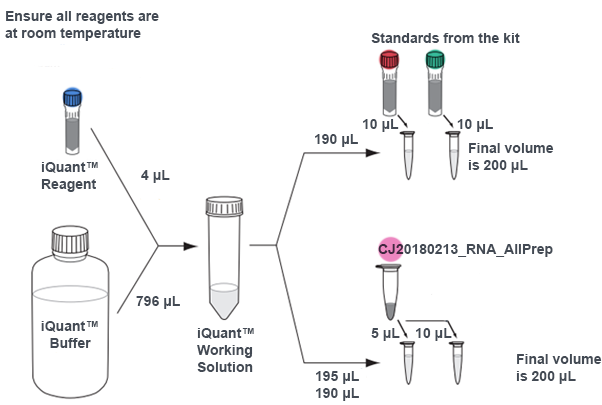
\includegraphics[width=\textwidth]{graphics/schemas/20180213_Qubit_assay_RNA.png}
        \caption{Qubit\texttrademark~ RNA BR assay}
        \label{sfig:20180213_Qubit_assay_RNA}
    \end{subfigure}
\end{figure}

\begin{table}[htbp]
\caption{Total DNA quantities in samples measured with Qubit RNA HS Assay Kit}
\label{tab:20180202_nuc_acid_qnt_dna}
\centering
\begin{tabular}{l l r r r r}
\toprule
 & Sample ID & \textmu g/mL & $V_f$ (mL) & m (\textmu g) & m (ng) \\ \midrule
DNA & \texttt{CJ20180213\_DNA} & 6.68 & 133.10\textsuperscript{-3} & 0.888 & 888.44 \\
DNA & \texttt{CJ20180213\_DNA} & 5.86 & 133.10\textsuperscript{-3} & 0.779 &  779.38 \\
\midrule
RNA & \texttt{CJ20180213\_RNA} & 34.6 & 63 .10\textsuperscript{-3} & 2.1798 &  \\
RNA & \texttt{CJ20180213\_RNA} & 31.5 & 63 .10\textsuperscript{-3} & 1.984 & 1984.5 \\
\bottomrule
\end{tabular}
\end{table}